%
% graph.tex
%
% (c) 2019 Prof Dr Andreas Müller, Hochschule Rapperswil
%
\begin{frame}[fragile]
\frametitle{Problem: Kürzeste Wege}
\begin{center}
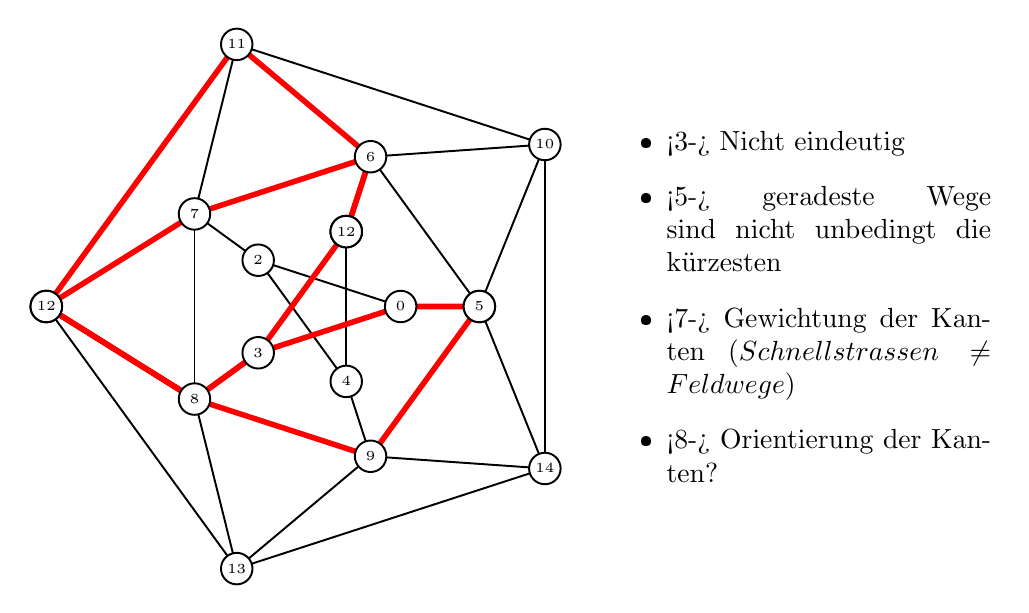
\begin{tikzpicture}[>=latex]

\def\blob#1#2#3{
	\fill[color=#3] #1 circle[radius=0.2];
	\draw[line width=0.7pt] #1 circle[radius=0.2];
	\node at #1 {{\tiny #2}};
}

\def\kante#1#2{
	\draw[line width=0.7pt,shorten >= 0.2,shorten >= 0.2] #1 -- #2 ;
}

\def\a{72}
\def\r{1.0}
\def\R{2.0}
\def\RR{3.5}

\coordinate (A1) at ({\r*cos(0*\a)},{\r*sin(0*\a)});
\coordinate (B1) at ({\r*cos(1*\a)},{\r*sin(1*\a)});
\coordinate (C1) at ({\r*cos(2*\a)},{\r*sin(2*\a)});
\coordinate (D1) at ({\r*cos(3*\a)},{\r*sin(3*\a)});
\coordinate (E1) at ({\r*cos(4*\a)},{\r*sin(4*\a)});

\coordinate (F1) at ({\R*cos(0*\a)},{\R*sin(0*\a)});
\coordinate (G1) at ({\R*cos(1*\a)},{\R*sin(1*\a)});
\coordinate (H1) at ({\R*cos(2*\a)},{\R*sin(2*\a)});
\coordinate (I1) at ({\R*cos(3*\a)},{\R*sin(3*\a)});
\coordinate (J1) at ({\R*cos(4*\a)},{\R*sin(4*\a)});

\coordinate (K1) at ({\RR*cos(0.5*\a)},{\RR*sin(0.5*\a)});
\coordinate (L1) at ({\RR*cos(1.5*\a)},{\RR*sin(1.5*\a)});
\coordinate (M1) at ({\RR*cos(2.5*\a)},{\RR*sin(2.5*\a)});
\coordinate (N1) at ({\RR*cos(3.5*\a)},{\RR*sin(3.5*\a)});
\coordinate (O1) at ({\RR*cos(4.5*\a)},{\RR*sin(4.5*\a)});

\kante{(A1)}{(C1)}
\kante{(C1)}{(E1)}
\kante{(E1)}{(B1)}
\kante{(B1)}{(D1)}
\kante{(D1)}{(A1)}

\kante{(F1)}{(G1)}
\kante{(G1)}{(H1)}
\kante{(H1)}{(I1)}
\kante{(I1)}{(J1)}
\kante{(J1)}{(F1)}

\kante{(A1)}{(F1)}
\kante{(B1)}{(G1)}
\kante{(C1)}{(H1)}
\kante{(D1)}{(I1)}
\kante{(E1)}{(J1)}

\kante{(K1)}{(L1)}
\kante{(L1)}{(M1)}
\kante{(M1)}{(N1)}
\kante{(N1)}{(O1)}
\kante{(O1)}{(K1)}

\kante{(F1)}{(K1)}
\kante{(G1)}{(L1)}
\kante{(H1)}{(M1)}
\kante{(I1)}{(N1)}
\kante{(J1)}{(O1)}

\kante{(F1)}{(O1)}
\kante{(G1)}{(K1)}
\kante{(H1)}{(L1)}
\kante{(I1)}{(M1)}
\kante{(J1)}{(N1)}

\uncover<2>{
	\draw[line width=2pt,color=red] (M1)--(H1)--(G1)--(B1);
}

\uncover<3>{
	\draw[line width=2pt,color=red] (M1)--(L1)--(G1)--(B1);
}

\uncover<4>{
	\draw[line width=2pt,color=red] (M1)--(I1)--(D1)--(B1);
}

\uncover<5>{
	\draw[line width=2pt,color=red] (M1)--(I1)--(D1)--(A1)--(F1);
}

\uncover<6->{
	\draw[line width=2pt,color=red] (M1)--(I1)--(J1)--(F1);
}

\uncover<2-4>{
	\blob{(B1)}{1}{red!20}
	\blob{(M1)}{12}{red!20}
}
\uncover<5-8>{
	\blob{(M1)}{1}{red!20}
	\blob{(F1)}{12}{red!20}
}

\blob{(A1)}{0}{white}
\uncover<1>{
	\blob{(B1)}{1}{white}
}
\uncover<5-8>{
	\blob{(B1)}{12}{white}
}
\blob{(C1)}{2}{white}
\blob{(D1)}{3}{white}
\blob{(E1)}{4}{white}
\uncover<1-4>{
	\blob{(F1)}{5}{white}
}
\blob{(G1)}{6}{white}
\blob{(H1)}{7}{white}
\blob{(I1)}{8}{white}
\blob{(J1)}{9}{white}
\blob{(K1)}{10}{white}
\blob{(L1)}{11}{white}
\uncover<1>{
	\blob{(M1)}{12}{white}
}
\blob{(N1)}{13}{white}
\blob{(O1)}{14}{white}

\node at (6,0) {\begin{minipage}{5cm}
\begin{itemize}
\item<3-> Nicht eindeutig
\item<5-> geradeste Wege sind nicht unbedingt die kürzesten
\item<7-> Gewichtung der Kanten
($\text{Schnellstrassen}\ne\text{Feldwege}$)
\item<8-> Orientierung der Kanten?
\end{itemize}
\end{minipage}};

\end{tikzpicture}
\end{center}
\end{frame}
